\section{Introduction}

Contemporary security identification has led to a plethora of biometric-based authentication systems. From palm readers at testing centers to facial recognition on smartphones, many systems are now used to regularly verify identities. These inherence-based systems are attractive in comparison to knowledge or possession-based methods of authentication because biometrics are highly unique, unforgettable, and far more difficult to steal than a password or swipe card.

Although biometric identification appears sophisticated when compared to something like physical keys, it does not come without its own share of caveats. For example, due to the ongoing Covid19 pandemic, many people wear masks when outside of their house, challenging most facial recognition systems. Additionally, biometrics that rely on touch, such as fingerprinting, raise safety concerns, as the scanner may become a vector for virus transmission. Despite these setbacks, given their merits and widespread deployment, biometric identification systems are unlikely to disappear.

One behavioral biometric that has gained recent success and is worth further consideration given current constraints is gait recognition. Usage of gait recognition has grown in the security industry in recent decades due to advances in deep learning. Singh et al. \cite{Singh2019APerspectives} categorized gait recognition into two main categories, vision-based and sensor-based. In vision-based approaches, cameras capture data of a person walking for the purpose of gait recognition. Sensor-based gait recognition is performed using either wearable sensors which produce kinematic data, or floor sensors which produce kinetic data \cite{Connor2018BiometricFeatures}.




This project uses two different datasets, Stepscan and UoM-Gait-Dataset. The UoM-Gait-Dataset was obtained from iMAGiMAT \cite{Cantoral-Ceballos2015IntelligentEnvironments}(an optical floor sensor). This sensor containing about 160 distributed \gls{pods} that indicate the foot pressure signals over time. Some studies like \cite{} use this dataset to construct an image for their research.

The second dataset that used for this project called Stepscan \cite{Connor2015ComparingBiometrics}. This dataset consists a spatial-temporal tensor, X, with dimensions $S × T × H × W$ where S represents the number of samples. T is the number of temporal observations, H and W are the dimension of image in pixels. Figure \ref{fig:training_data} indicates the this tensor in two various time for a sample.

\begin{figure}[]
    \centering
    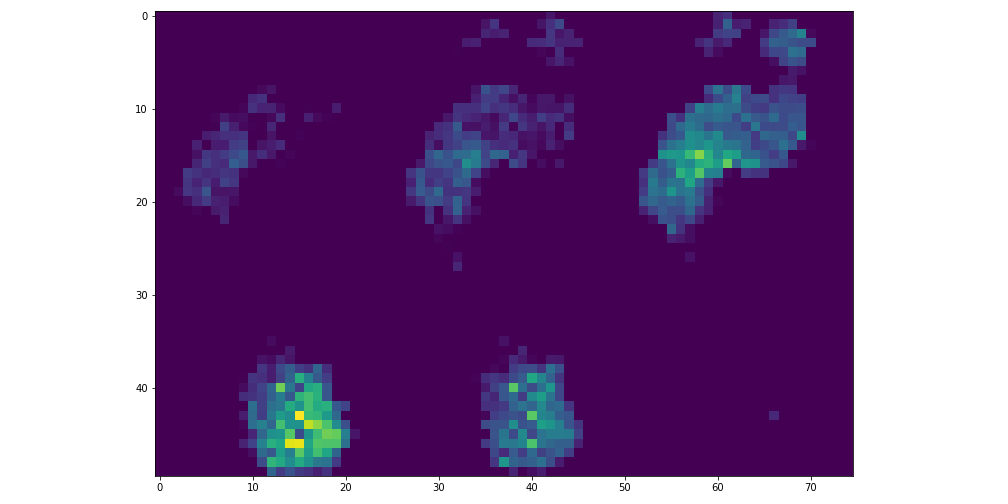
\includegraphics{figures/project/frame1.png}
    \caption{different time observation of a footprint images in the Stepscan dataset.}
    \label{fig:Stepscan_dataset}
\end{figure}


containing the spatial footprint

For changing the images to time series data, there are two methods. In the first method, the values of each pixel over time consider as a time series. As a result for each sample, This method produce $H × W$ time series.

In the second method, some spatial features extract from each image (e.g. mean function) and show their changes over time. Therefore, 2D images ($H × W$) is reduce to one value.

As the figure \ref{fig:training_data} shows the data is a image not a time series data. Therefore we need to convert our data to a time series. 


%CASIA-D, a kinetic gait dataset captured by arrays of high-quality pressure sensors. The dataset consists of multiple footprint images from 88 participants (20 female and 68 males) between 20 and 60 years old [3]. Participants each completed ten unshod walking trials. Each trial produced three footprint images for a total of 30 images per participant. These images are the combination of many readings as different parts of the participants' feet are in contact with the sensors. Stitching these readings together has produced pictures of participants' bare feet (see Figure 1). Half the trials were completed at a subjectively slow walking pace, (15 images) and the other half at a subjectively fast pace.

This project explored three scenarios for classification and prediction of subjects.
%identification using gait data. Several classifiers and feature types are compared to attain the best possible accuracy using the CASIA-D dataset. These classifiers include LDA, QDA, kNN and SVM all classifying manually extracted footprint features. Image based classification is attempted using PCA reduction and eigenvectors. Convolutional neural networks (CNNs) are also employed for feature generation and classification. Finally, two subproblems are attempted. The first being an exploration of the effects of walking speed on classification. The second attempts to objectify how symmetrical participant’s left and right foot images are.